\documentclass{article}

\usepackage[latin1]{inputenc}
\usepackage{mathtools}
\usepackage{graphicx}
\usepackage{float}
\usepackage{setspace}
%\doublespacing

%%%%%%%%%%%%%%%% Lengths %%%%%%%%%%%%%%%%
\setlength{\textwidth}{15.5cm}
\setlength{\evensidemargin}{0.5cm}
\setlength{\oddsidemargin}{0.5cm}

%%%%%%%%%%%%%%%% Variables %%%%%%%%%%%%%%%%
\def\projet{5}
\def\titre{Interpolation and integration methods / Cubic splines and surface interpolation}
\def\groupe{2}
\def\equipe{1}
\def\responsible{cbroc}
\def\secretary{htoussaint}
\def\others{rpetro, pmeyzen, amilliet}

\begin{document}

%%%%%%%%%%%%%%%% Header %%%%%%%%%%%%%%%%
\noindent\begin{minipage}{0.98\textwidth}
  \vskip 0mm
  \noindent
  { \begin{tabular}{p{7.5cm}}
      {\bfseries \sffamily
        Project n�\projet} \\ 
      {\itshape \titre}
    \end{tabular}}
  \hfill 
  \fbox{\begin{tabular}{l}
      {~\hfill \bfseries \sffamily Group n�\groupe\ - Team n�\equipe
        \hfill~} \\[2mm] 
      Responsible : \responsible \\
      Secretary : \secretary \\
      Programmers : \others
    \end{tabular}}
  \vskip 4mm ~

  ~~~\parbox{0.95\textwidth}{\small \textit{Summary~:} \sffamily The aim of this project was to implement a model representing the airflow around an airfoil. More precisely, a pressure map below and above the wing was to be computed, so as to approximate the ability of a plane to remain in the air. This was achieved through three steps. First the airfoil was refined into a sufficiently smooth curve, using cubic splines. Then the length of the curve had to be computed, using integration methods. Finally the airflow was modelled using a laminar model, and a map describing the pressure around the airfoil was computed.  }
  \vskip 1mm ~
\end{minipage}

%%%%%%%%%%%%%%%% Main part %%%%%%%%%%%%%%%%
\section*{Airfoil refinement}
The first part was aimed at refining the airfoil, consisting of a list of points, into a sufficiently smooth curve. First, an airfoil profile was arbitrarily selected from the UIUC database, and loaded as arrays of points, using a python function provided (load\_foil). Then the several measurements of the  airfoil were split into two parts representing the upper surface and the lower surface of the wing.\\

The variables returned by this function correspond to the abscissas and ordinates of the points of both the upper surface ($ex$ and $ey$) and the lower surface ($ix$ and $iy$). The data, stored in arrays (as previously stated), were used to draw the curves describing the airfoil.\\

The curves had then to be sufficiently smoothed to be properly used and easily integrated. This was achieved through cubic spline interpolation. A piecewise-polynomial curve joins the points of a given set, such that each polynomial equation between each point is at most of order 3, and such that the continuity, the first and the second derivative of the overall curve is preserved.\\

At first, a scipy function (interp1d) was used to compute the interpolation to get a display of the expected result (figure 1).\\

Then, a proper function had to be programmed, with the help of the functions and explanations given in the Numerical Recipes (spline and splint).

\begin{figure}[H]
  \begin{center}
  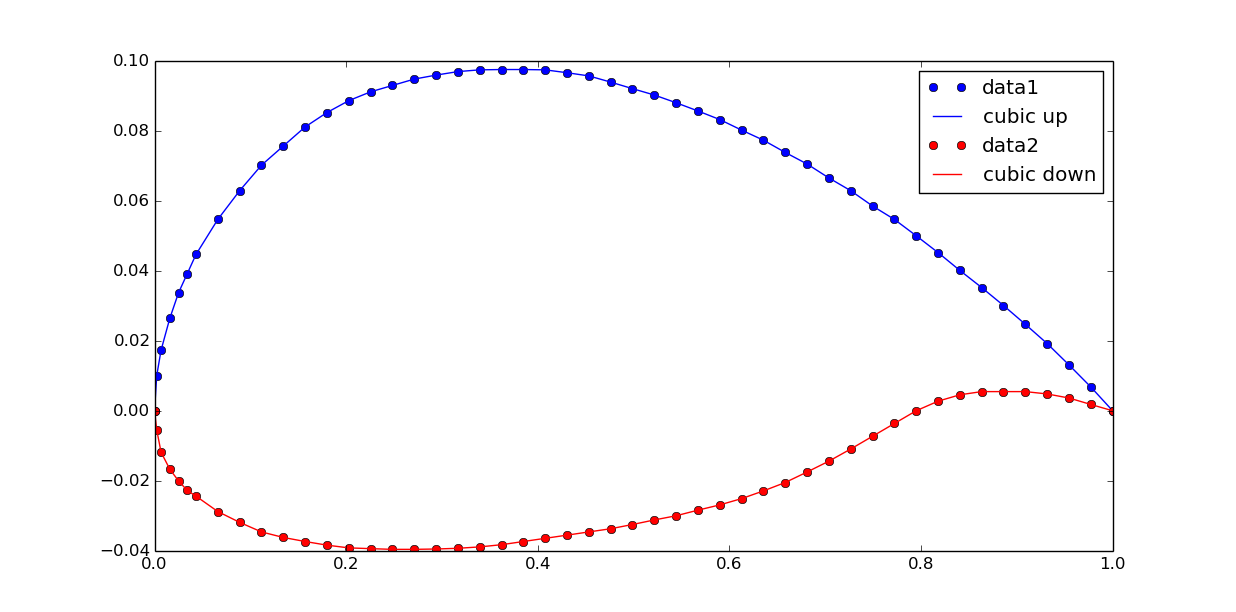
\includegraphics[scale=0.5]{figure_1.png}
  \end{center}
  \caption{Cubic spline interpolation of the upper (blue) and lower (red) surfaces}
\end{figure}





\section*{Computing the length of plane curves}

Thanks to the cubic splines we were able in the first part to get a continuous function from several points around the airfoil.
In this part, the aim was to compute the length of the curve, in order to obtain a pressure map in the last part of this project.
The splines are given as a function $x\rightarrow f(x)$, which has been provided by cubic splines in the previous section, and the length of the curve can be calculated by the following integral:\\
\begin{equation}
L([0;T]) = \displaystyle \int_0^T     \sqrt{1+f'(x)^2} ~dx
\end{equation}

First of all, the derivative of the function f had to be computed. The code of this function is called ``differentiation(x,eps)'' and is given in the source code. The derivative was calculated on several given points, which is why the first input ``x'' is a table. The second input ``eps'' is the step used to determine the derivative on each point.\\

Then, the length of the curve was computed by the function named ``curve\_length(integ\_method,f,a,b,n)'' where $f$ is a continuous function provided by cubic splines, as previously described, a and b are the bounds of an interval, and n is the number of subsystems in this interval.\\

Three integration methods were computed in this project so the user had to be able to choose one of them.
In order to produce a generic tool, the integration method is a parameter of the function length, so the user can choose the method he wants to use to determine the length of the plane.\\

The first integration method implemented is the rectangle rule. This method consists in dividing the interval $[a,b]$ over which the function is to be integrated into $n$ equal subintervals of length $l$. The surface under the curve is then divided into rectangles of equal length l and whose heights are determined by the values of the function.
More specifically, the rectangles can be placed so that their left or right upper corner, or the middle of their top lign is exactly on the curve.
In the case of the upper right corner, the integral is approximated by the following formula (using the parameters previously defined):
\begin{equation}
\displaystyle \int_a^b f(x)\,dx \approx l \sum_{k=1}^{n} f(a+kh)
\end{equation}

A second method called trapezoidal rule was also programmed in this project. The interpolation function is a first order polynomial. The quadrature used to approximate the integral is the following:
\begin{equation}
\displaystyle I\approx h(\tfrac{f(a)-f(b)}{2} + \sum_{k=1}^{n-1} f(a+kh))
\end{equation}

Finally the Simpson rule was the third integration method implemented in our project. It consists in interpolating a function with a second order polynomial. The quadrature is the following:
\begin{equation}
\displaystyle I\approx h(\tfrac{f(a)+f(b)}{6} + \sum_{k=1}^{n-1}\tfrac{1}{3}f(a+kh) + \sum_{k=0}^{n-1}\tfrac{2}{3}f(a+kh+\tfrac{h}{2})
\end{equation}

\section*{Modelling the airflow}
After having drawn the shape of the airfoil and calculated the length of its curve, the goal of the last part was to model the behaviour of the airflow above and below the wing, following a laminar model, and to draw a pressure map of the air around the wing.\\

The modelling of the airflow was computed following the instructions given in the subject.
Every slice is given by the following function :
\begin{equation}
y = f_{\lambda}(x) = (1-\lambda)f(x)+\lambda    \times 3h_{max} \qquad \forall \lambda \in [0;1]
\end{equation}
Each slice matches a certain value of $\lambda$.
In our example, $h_{max} \approx 0.10$ and $h_{min} \approx -0.04$, and 20 slices were drawn, as shown in figure 2.

\begin{figure}[H]
  \begin{center}
  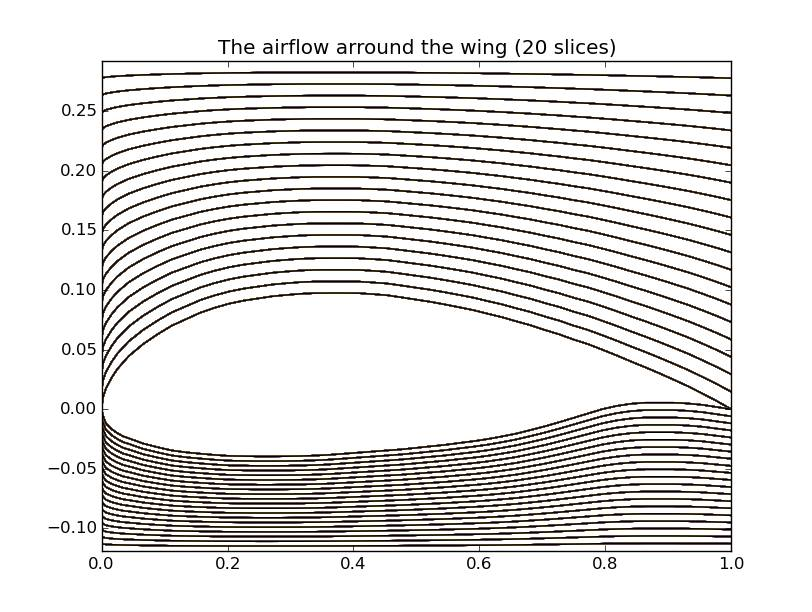
\includegraphics[scale=0.35]{figure_2.jpg}
  \end{center}
  \caption{Laminar flow above and below the airfoil}
\end{figure}

Finally, in order to draw the pressure map of the air above and below the wing, a matrix containing the values of the pressure at each point had to be computed, using the formula given in the instructions (the Bernoulli law). The pressure is indeed proportional to the speed squared. Moreover, on each slice of the laminar flow, the pressure is equal on every point of the slice. For example, on every point of the slice closest to the upper side of the airfoil, the pressure is equal and maximal.\\

This is where the length of the curve calculated in the previous section comes into use. The speed is calculated by computing the length of each slice, represented by the aforementioned $f_{\lambda}$ functions. The closer the slices are from the airfoil , the sharper and longer they get, and the longer they are, the higher the speed of the airfoil is.
The pressure map obtained in the end is given in the following figure:

\begin{figure}[H]
\centering
\begin{minipage}{.5\textwidth}
  \centering
  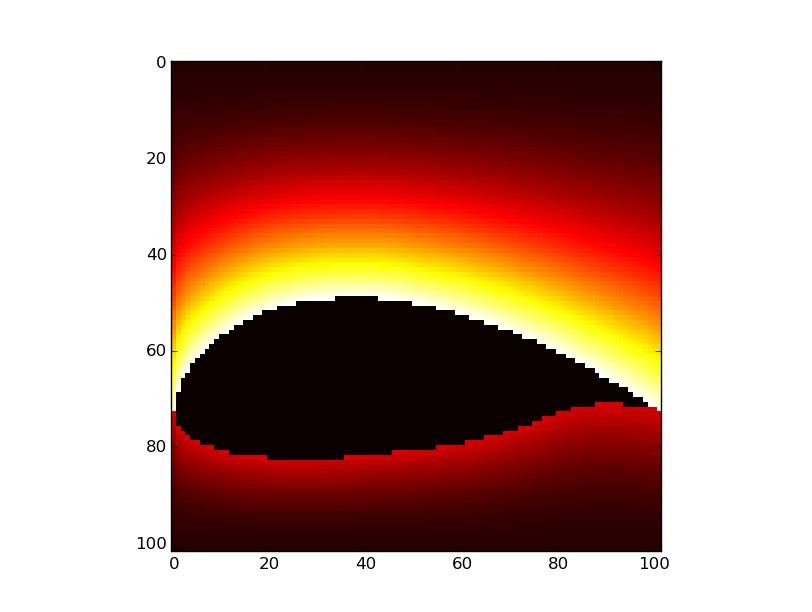
\includegraphics[width=1\linewidth]{figure_3-1.jpg}
\end{minipage}%
\begin{minipage}{.5\textwidth}
  \centering
  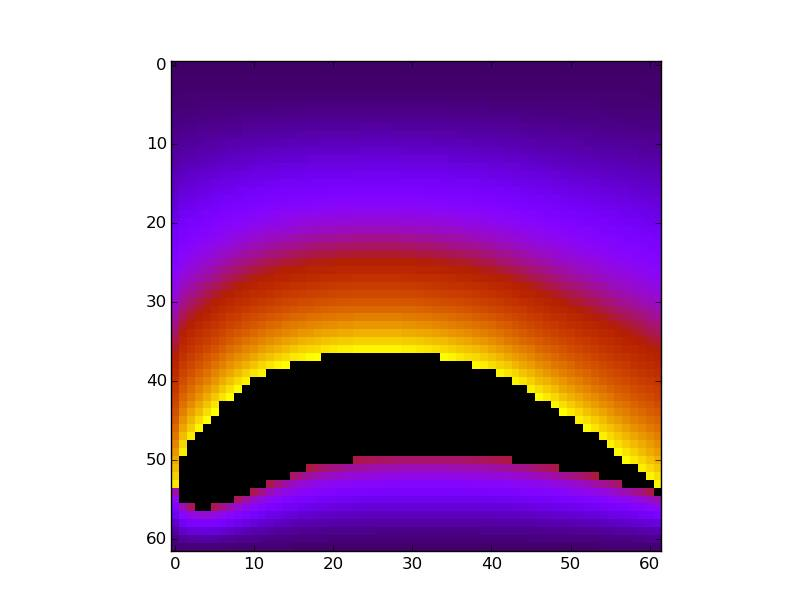
\includegraphics[width=1\linewidth]{figure_3-2.jpg}
\end{minipage}
\caption{Pressure maps of two different airfoil, using two different color schemes}
\end{figure}

\subsection*{Conclusion}

As can be seen on the maps (figure 3), the pressure is highest right above the airfoil. Due to the high pressure difference, the wing is pulled upward. The previous principle explains how an airplane remains in the air, which was the implicit goal of the project.
\end{document}

